\documentclass[10pt,a4paper]{article}
\usepackage[utf8]{inputenc}
\usepackage[T1]{fontenc}
\usepackage{lmodern}
\usepackage[margin=1.5cm, top=1.4cm, bottom=1.4cm]{geometry}
\usepackage{hyperref}
\usepackage{enumitem}
\usepackage{titlesec}
\usepackage{xcolor}
\usepackage{graphicx}

\definecolor{accent}{HTML}{00686E}
\hypersetup{colorlinks=true, urlcolor=accent, linkcolor=accent}
\pagenumbering{arabic}
\setlength{\parindent}{0pt}

\titleformat{\section}{\large\bfseries\color{accent}}{}{0em}{}[\vspace{-0.6em}\rule{\textwidth}{0.8pt}]
\titlespacing{\section}{0pt}{7pt}{4pt}

\newcommand{\role}[4]{%
  \textbf{#1} \hfill \textbf{#2}\\[1pt]%
  \textit{#3} \hfill \textit{#4}\\[2pt]%
}
\setlist[itemize]{leftmargin=1.2em, itemsep=1.5pt, topsep=2pt, parsep=0pt}

\begin{document}

% ================= HEADER =================
\begin{minipage}[c]{0.80\textwidth}
  {\Huge\bfseries Prabhavit Gupta}\\[3pt]
  {\color{accent}\large Senior Solutions Engineer: Frontend Tooling, Developer Platforms \& Integrations}\\[6pt]
  {\footnotesize +39 351 610 7807 ~$\vert$~
  \href{mailto:prabhavitg@gmail.com}{prabhavitg@gmail.com} ~$\vert$~
  \href{https://www.linkedin.com/in/prabhavit/}{linkedin.com/in/prabhavit} ~$\vert$~
  \href{https://github.com/prab-gupta}{github.com/prab-gupta} ~$\vert$~
  Venice, Italy}
\end{minipage}\hfill
\begin{minipage}[c]{0.18\textwidth}
  \raggedleft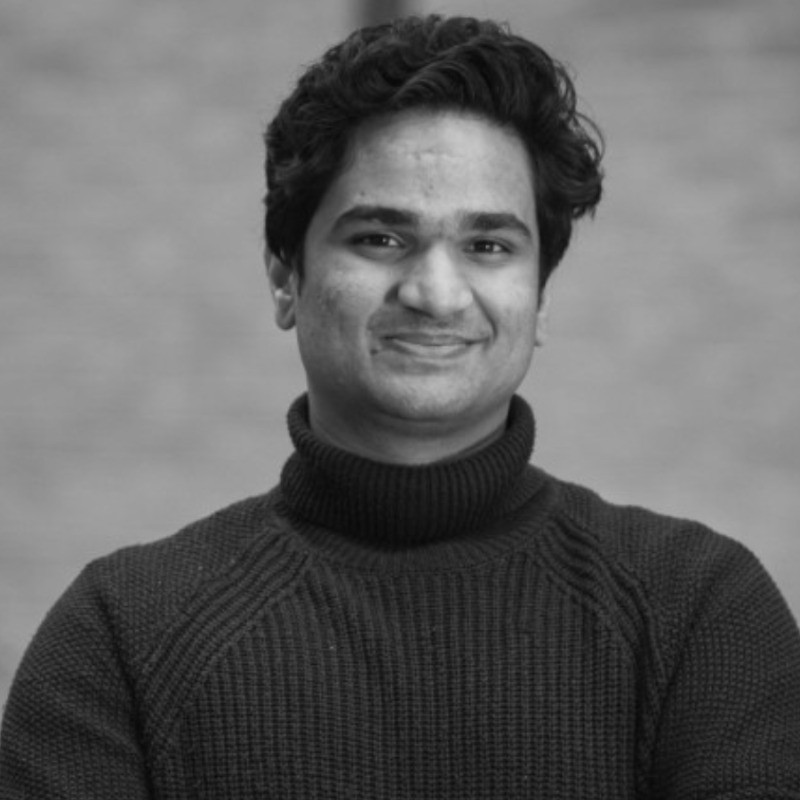
\includegraphics[width=2.0cm]{photo.jpg}
\end{minipage}
\vspace{-2pt}

% ================= SUMMARY =================
\section{Summary}
Solutions and Integration Engineer with 3 years of hands-on experience delivering customer-facing technical solutions, developer platform tooling, and modern frontend architectures across European tech teams. At FlowSpace, led platform migration to Next.js, React, and TypeScript, engineered automated end-to-end regression suites with Playwright, and integrated multi-tenant enterprise APIs with idempotent webhook synchronization. Experienced in diagnosing subtle frontend and integration issues across build pipelines, Webpack configurations, and CI/CD environments. Proven track record guiding enterprise stakeholders from initial discovery through technical onboarding and production adoption. Based in Venice, Italy with an EU Long Term Residence Permit (unrestricted EU work authorization without sponsorship). Immediately available.

% ================= TECHNICAL EXPERTISE =================
\section{Technical Expertise}
\begin{itemize}
  \item \textbf{Frontend \& Component Tooling:} TypeScript, JavaScript, React, Next.js, Webpack, Vite, Storybook, Chromatic, CSS/Tailwind, DOM APIs, Cross-browser debugging.
  \item \textbf{Testing \& Automation:} Playwright, Automated visual regression testing, CI/CD pipelines (GitHub Actions), End-to-end test harnesses, n8n, Webhooks.
  \item \textbf{Solutions Engineering:} Technical discovery, Enterprise customer onboarding, Tailored proof-of-concept (POC) builds, Troubleshooting ambiguous production issues, Account expansion support.
  \item \textbf{Full Stack \& Infrastructure:} Node.js, Working-level Python, Laravel, RESTful APIs, WebSockets, Supabase, PostgreSQL, Docker, Git.
  \item \textbf{Languages \& Work Authorization:} Hindi (Native), English (C1 Professional), Italian (Beginner). EU Long Term Residence Permit (Permanent unrestricted EU work authorization; no visa sponsorship required).
\end{itemize}

% ================= EXPERIENCE =================
\section{Experience}

\role{\href{https://flowspace.co}{FlowSpace.co}}{Mar 2024 - Aug 2026}{Lead Developer (Full-time, Freelance)}{London, UK (remote)}
\begin{itemize}
  \item Directed full-stack platform migration to modern Next.js, React, and TypeScript, establishing component-driven UI standards and maintainable architecture.
  \item Built and maintained comprehensive automated test suites using Playwright to catch regressions across user-facing checkout, booking, and administrative workflows.
  \item Served as the primary technical interface for B2B space partners, guiding onboarding, configuring API integrations, and troubleshooting production sync discrepancies.
  \item Resolved complex edge-case synchronization issues between external management systems (OfficeRnD, Nexudus) and internal databases using idempotent webhook reconciliation.
  \item Architected and deployed production customer support AI agents using LLM tool calling and live REST API function calling to query platform availability and execute bookings.
  \item Built an automated knowledge ingestion pipeline: parsed heterogeneous documents (PDFs, spreadsheets, web pages) into structured database records, creating 900+ verified listings.
  \item Scaled platform user base from 2,000 to 4,500+ active users through iterative product engineering and resilient frontend automations.
\end{itemize}

\role{Urlink}{Apr 2025 - Jul 2025}{Project Manager \& AI Assisted Developer (Freelance)}{Barcelona, Spain (remote)}
\begin{itemize}
  \item Led technical delivery of AI-assisted web applications, coordinating API contracts, database schemas, and frontend component integration.
  \item Implemented automated CI/CD checks and test suites, ensuring clean code releases and minimal deployment regressions.
  \item Evaluated commercial LLM APIs across task types, optimizing prompt structures and model selection for latency and output consistency.
\end{itemize}

\role{Independent Technical Consultant}{Aug 2023 - Feb 2024}{AI Solutions \& Automation Engineer}{Venice, Italy}
\begin{itemize}
  \item Developed custom web automations, integration prototypes, and data extraction pipelines for European SME clients using TypeScript, Playwright, and APIs.
  \item Provided technical consulting and hands-on onboarding to non-technical business founders, translating operational friction into automated software solutions.
  \item Implemented webhook listeners and data synchronization flows, replacing manual administrative processes.
\end{itemize}

% ================= EDUCATION =================
\section{Education}
\role{Ca' Foscari University of Venice}{2020 - 2024}{BA in Philosophy, International Studies and Economics}{Venice, Italy}
\begin{itemize}
  \item In-depth focus on formal logic, analytical problem solving, systems analysis, and macroeconomic decision models.
\end{itemize}

\end{document}
